\chapter{Informações complementares}

\section*{Uso e manuseio do Óxido Nitroso}

\begin{center}
ATENÇÃO
    \begin{figure}[H]
\centering
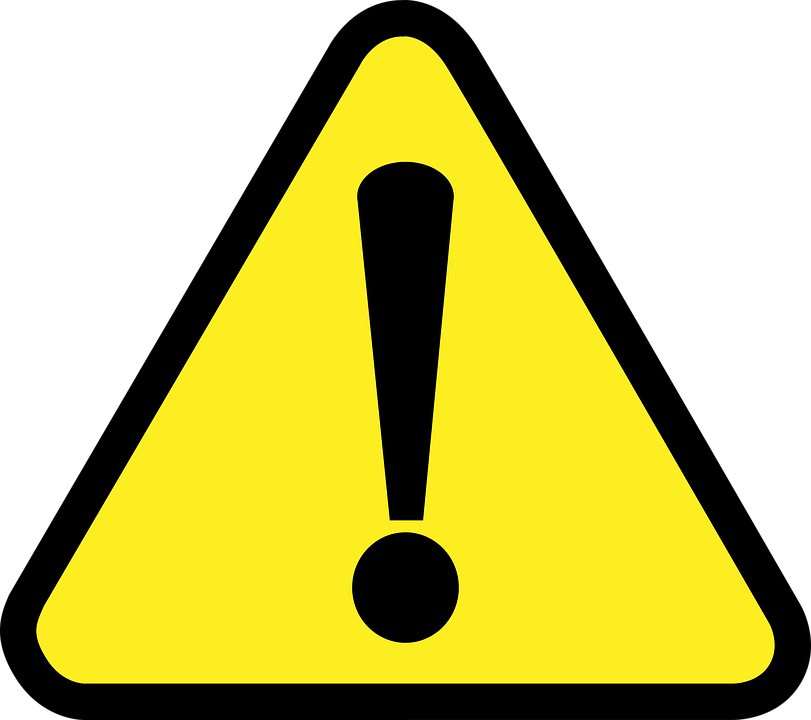
\includegraphics[scale = 0.1]{Figuras/atenção.png}
\end{figure}
\end{center}

\par O Óxido Nitroso é um gás não tóxico e não irritante com um efeito anestésico moderado e pode ser inalado misturado com oxigênio ou ar. Quando inalado sem oxigênio age como um asfixiante simples. No Brasil a Norma Regulamentadora 15 (NR 15), considera o produto como asfixiante simples e não impõe limites de exposição, entretanto, deve-se garantir que a concentração mínima de oxigênio seja de 18\% em volume. 

\par O sistema não vem com o cilindro de óxido nitroso, porém entende-se que o usuário que adquirir o produto estará lidando com esse tipo de propelente. Dessa forma para a segurança do cliente e correto manuseio de todas as partes do sistema indica-se a leitura dos protocolos de segurança estabelecidos para o uso e manuseio do óxido nitroso. Como fonte de referencia indica-se o seguinte \href{https://www.airliquidehealthcare.com.br/sites/alh_br/files/23003_oxido_nitroso_liquido_refrigerado10024-97-2.pdf}{link} de leitura.

\section*{Documentação técnica}

\par O seguinte produto é de desenvolvimento educacional, com caráter pre-eliminar e de prototipagem. Sua documentação técnica e de desenvolvimento encontram-se disponíveis para acesso através do repositório desenvolvido pelo grupo. 

\par Todas as informações encontram-se devidamente documentadas no relatório de desenvolvimento e seus aspectos de construção detalhados em seu manual de montagem.

\par É proibida a produção e venda deste sem autorização dos direitos intelectuais por parte do grupo desenvolvedor.

\section*{Descarte correto do equipamento}

    \begin{figure}[H]
    \centering
		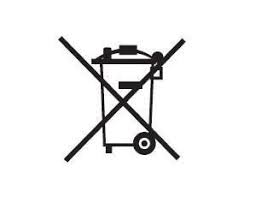
\includegraphics[scale=1]{Figuras/lixo.jpg}
    \end{figure} 
    
\par Resíduos de equipamentos Elétricos e Eletrônicos não deverão ser descartados juntamente com os resíduos domésticos. Assim como as baterias não devem ser descartadas com o lixo doméstico no final de sua vida útil. Isso se dá para impedir danos ao ambiente ou à saúde pública causados pelo descarte indevido de resíduos. Dessa forma você deverá separar estes equipamentos de outros tipos de resíduos e reciclá-los de forma responsável, de modo a promover uma reutilização sustentável dos recursos materiais.
\begin{center}
A equipe desenvolvedora apoia o seguinte movimento:
     \begin{figure}[H]
    \centering
		
\includegraphics[scale=0.5]{Figuras/lixo_eletronico.jpg}
    \end{figure} 
\end{center}
